\section{Theorie}
\label{sec:Theorie}

        \subsection{Wechselwirkung von \texorpdfstring{$\gamma-$}\,Quanten mit Materie}

            Trifft ein $\gamma-$Quant auf Materie, treten im Wesentlichen 
            drei Arten von Wechselwirkung auf: Photoeffekt, Comptoneffekt 
            und Paarbildung. Die Absorptionskoeffizienten der einzelnen 
            Wechselwirkungen sind stark von der Photonenenergie abhängig,
            sodass in unterschiedlichen Energiebereichen unterschiedliche
            Effekte dominieren. Dies wird in Abb.~\ref{fig:blei} am Beispiel
            von Blei gezeigt, in welcher die einzelnen Absorptionskoeffizienten 
            eingezeichnet sind und
            auch der resultierende totale Absorptionskoeffizient zu sehen ist.

            \begin{figure}
                \centering
                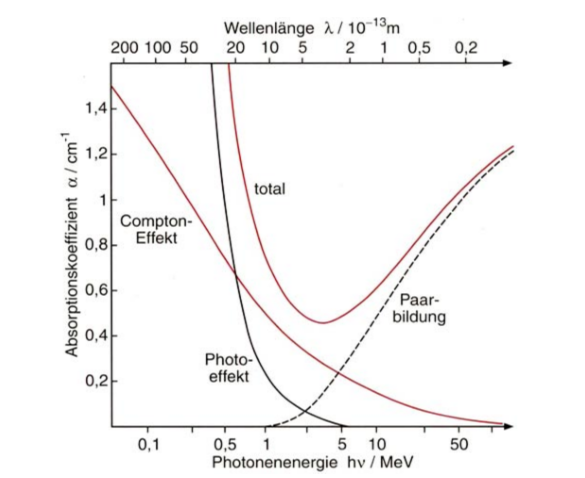
\includegraphics{blei.png}
                \caption{Absorptionskoeffizienten von Blei für die drei wesentlichen 
                Wechselwirkungen von $\gamma-$Quanten mit Materie mit eingezeichnetem 
                resultierenden absoluten Absorptionskoeffizienten \cite{blei}.}
                \label{fig:blei}
            \end{figure}

            \subsubsection{Photoeffekt}

                Trifft ein $\gamma-$Quant auf ein Hüllenelektron und ist seine 
                Energie größer als dessen Bindungsenergie, wird das Elektron 
                aus der Schale herausgelöst. Der Quant wird dabei vernichtet, 
                da die übrige Energie des Quants in kinetische Energie des Elektrons
                umgewandelt wird. Elektronen, welche zurückfallen, um die Löcher 
                in den Schalen zu schließen, senden ihrerseits $\gamma-$Quanten aus,
                welche in der Regel im Absorber verbleiben. Der Photoeffekt ist 
                bei kleinen Photonenergien der dominierende Wechselwirkungseffekt, 
                bei Blei dominiert er z.B. bis zu Energien von etwa 1\,MeV.


            \subsubsection{Comptoneffekt}

                Beim Compton-Effekt wird der Quant an einem quasi-ruhenden Elektron gestreut
                und überträgt ihm einen Teil seiner Energie. Der $\gamma-$Quant ändert dabei 
                seine Richtung und vergrößert seine Wellenlänge. Er kann bei diesem Vorgang nie 
                vollständig vernichtet werden. Der Comptoneffekt tritt bereits für kleine Photonenenergien
                auf, ist aber erst dann der dominierende Effekt, wenn der Einfluss des Photoeffekts sinkt. 
                Dies ist bei Blei zwischen etwa 1 und 5\,MeV der Fall.

            \subsubsection{Paarbildung}

                Paarbildung wird erst ab sehr hohen Quantenergien (>5\,MeV) relevant.
                Die Energie muss dabei größer sein als die doppelte Ruhemasse 
                des Elektrons. Unter diesen Umständen ist es möglich, dass sich der 
                Quant in ein Elektron und ein Positron umwandelt. Im Experiment ist 
                der Prozess der Paarbildung jedoch nicht von Bedeutung, da der hierzu 
                erforderliche Energiebereich nicht betrachtet wird.

        \subsection{Szintillatoren}

            Mithilfe von Szintillatoren können radioaktive Teilchen und Strahlungen nachgewiesen werden.
            In diesem Versuch wird ein NaJ-Szintillator zum Nachweis von Gammaquanten verwendet, 
            welche durch Anregung des Szintillatormaterials die Entstehung von Lichtblitzen verursachen.
            Diese Lichtblitze werden in Photomultipliern in elektronische Signale umgewandelt
            und verstärkt, wobei die Signalhöhe linear mit der Quantenenergie zusammenhängt. 
            Es gibt zwei Typen von Szintillatormaterialien: Organische und Anorganische.
            Organische Szintillatormaterialien haben den Vorteil einer schnellen Zerfallszeit, welche im 
            Bereich von Nanosekunden liegt. Anorganische Szintillatoren, zu denen auch der im Versuch 
            verwendete zählt, haben eine deutlich langsamere Zerfallszeit im Bereich von einigen 
            hundert Nanosekunden. Vorteilhaft an dieser Szintillatorart ist ihre hohe Dichte und 
            Ordnungszahl, da dadurch mehr Gammaquanten detektiert werden können und somit die 
            Energieauflösung erhöht wird.


        \subsection{Tomographie}

            In der Tomographie wird $\gamma-$Strahlung durch einen Körper oder Gegenstand geleitet.
            Anhand der Abschwächung können Rückschlüsse auf das Material getroffen werden. 
            Durchläuft der Strahl hintereinander mehrere Materialien, ergibt sich die Endintensität zu

            \begin{align*}
                N = I_0 \,e^{-\sum\mu_id_i}.
            \end{align*}
            Dabei bezeichnet $I_0$ die Eingangsintensität, $\mu_i$ und $d_i$ sind Absorptionskoeffizient
            bzw. Dicke des $i$-ten Materials. Aus der $j-$ten Endintensität $N_j$ und der Eingangsintensität 
            kann die $j-$te Projektion $I_j$ berechnet werden durch

            \begin{align*}
                I_j = \symup{ln}\left(\frac{I_0}{N_j}\right).
            \end{align*}
            Für eine 3\,x\,3\,-Würfelschicht, welche im Experiment untersucht wird, müssen mindestens neun 
            Projektionen aufgenommen werden, um ein Gleichungssystem aufstellen zu können, dessen Lösung 
            die neun Materialien der neun Elementarwürfel darstellt. 
            \begin{figure}
                \centering
                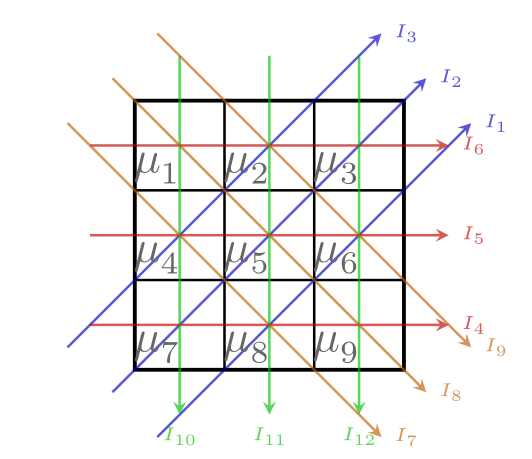
\includegraphics[height=5cm]{wuerfel.png}
                \caption{Richtungen der zwölf aufgenommenen Projektionen \cite{wuerf}.}
                \label{fig:wuerfel}
            \end{figure}
            Da Überbestimmung die Genauigkeit des 
            Ergebnisses verbessert, werden für diese Schicht 12 Projektionen aufgenommen 
            (siehe Abb.~\ref{fig:wuerfel}), sodass folgendes überbestimmtes Gleichungssystem entsteht:

        \begin{equation}
            d\cdot
            \begin{pmatrix}
                 0       &     0     &    0      &      0     &        0    & \sqrt{2} &    0      &  \sqrt{2} &           0 \\
                 0       &     0     &  \sqrt{2} &      0     &    \sqrt{2} &    0     &  \sqrt{2} &     0     &           0 \\
                 0       &  \sqrt{2} &    0      &   \sqrt{2} &        0    &    0     &    0      &     0     &           0 \\
                 0       &     0     &    0      &      0     &        0    &    0     &    1      &     1     &           1 \\
                 0       &     0     &    0      &      1     &        1    &    1     &    0      &     0     &           0 \\
                 1       &     1     &    1      &      0     &        0    &    0     &    0      &     0     &           0 \\
                 0       &     0     &    0      &   \sqrt{2} &        0    &    0     &    0      &  \sqrt{2} &           0 \\
              \sqrt{2}   &     0     &    0      &      0     &    \sqrt{2} &    0     &    0      &     0     &    \sqrt{2} \\
                 0       & \sqrt{2}  &    0      &      0     &        0    & \sqrt{2} &    0      &     0     &           0 \\
                 1       &     0     &    0      &      1     &        0    &    0     &    1      &     0     &           0 \\
                 0       &     1     &    0      &      0     &        1    &    0     &    0      &     1     &           0 \\
                 0       &     0     &    1      &      0     &        0    &    1     &    0      &     0     &           1 \\   
             \end{pmatrix}
             \cdot
             \begin{pmatrix}
                \mu_1\\
                \mu_2\\
                \mu_3\\
                \mu_4\\
                \mu_5\\
                \mu_6\\
                \mu_7\\
                \mu_8\\
                \mu_9\\
             \end{pmatrix}
             =
             \begin{pmatrix}
                I_1\\
                I_2\\
                I_3\\
                I_4\\
                I_5\\
                I_6\\
                I_7\\
                I_8\\
                I_9\\
                I_{10}\\
                I_{11}\\
                I_{12}\\
             \end{pmatrix}
             =  \textbf{A} \cdot \vec{\mu}
        \end{equation}
        Mithilfe der Methode der kleinsten Quadrate 
        kann die Gleichung umgeschrieben werden zu 
        \begin{align*}
            \vec{\mu} = (\textbf{A}^T\textbf{A})^{-1}\cdot\textbf{A}^T\cdot\vec{I}.
        \end{align*}
        Für den Fall gleicher Unsicherheiten ergeben sich die Varianzen zu 
        \begin{align*}
            \sigma_i^2 = \sigma_I^2\,\text{diag}[(\textbf{A}^{T}\textbf{A})^{-1}].
        \end{align*}